%
% File: chap01.tex
%
\let\textcircled=\pgftextcircled
\chapter{Flux in the core}
\label{chap:intro}

\initial{S}everal exercises from the book written by M. M. El Wakil~\cite{book01} are tackled in this homework. The problems in this section relate mostly to the third chapter of the book, covering the subject of the neutron flux distribution in cores.

%=======
\section{Finite cylinder}
\label{prob31}

\subsection{Problem}
\textit{Find the flux in a finite cylinder of radius $R$ and height $H$ using the diffusion theory.}

\subsection{Solution}

The diffusion equation can be written following Equation~\ref{eq31}.

\begin{equation}\label{eq31}
\nabla^2 \phi + B^2\phi = 0
\end{equation}

In a cylindrical coordinates system, the Laplacian $\nabla$ can be explicited according to Equation~\ref{eq32}.

\begin{equation}\label{eq32}
\nabla^2 \phi = \frac{\partial^2}{\partial r^2} + \frac{1}{r}\frac{\partial}{\partial r} + \frac{\partial^2}{\partial z^2}
\end{equation}

Consequently, we can rewrite Equation~\ref{eq31} to obtain Equation~\ref{eq33}.


\begin{equation}\label{eq33}
\frac{\partial^2 \phi(r, z)}{\partial r^2} + \frac{1}{r}\frac{\partial \phi(r, z)}{\partial r} + \frac{\partial^2 \phi(r, z)}{\partial z^2} + B^2\phi(r, z) = 0
\end{equation}

In order to solve this differential equation, one assumes that the axial flux component is independent from the radial flux component. In this case, the variables can be separated, using Definition~\ref{eq34}.


\begin{equation}\label{eq34}
\phi(r, z) = \rho(r)\zeta(z)
\end{equation}

This implies Equation~\ref{eq35}.


\begin{equation}\label{eq35}
\zeta(z)\frac{\partial^2 \rho(r)}{\partial r^2} + \frac{\zeta(z)}{r}\frac{\partial \rho(r)}{\partial r} + \rho(r)\frac{\partial^2 \zeta(z)}{\partial z^2} + B^2\rho(r)\zeta(z) = 0
\end{equation}

Now, it is useful to divide the equation by $\rho(r)\zeta(z)$ in order to isolate the $r$-component from the $z$-component, as seen in Equation~\ref{eq36}.


\begin{equation}\label{eq36}
\frac{1}{\rho(r)}\frac{\partial^2 \rho(r)}{\partial r^2} + \frac{1}{r\rho(r)}\frac{\partial \rho(r)}{\partial r} + \frac{1}{\zeta(z)}\frac{\partial^2 \zeta(z)}{\partial z^2} = -B^2
\end{equation}

Now, we have an equation of the form $f(x) + g(y) = cst$. This equation can only be verified if $f(x) = cst$ and $g(y) = cst$. Consequently, we have the following system of equations~\ref{eq37} and~\ref{eq38} to solve.

\begin{alignat}{2}
\frac{1}{\rho(r)}\frac{\partial^2 \rho(r)}{\partial r^2} + \frac{1}{r\rho(r)}\frac{\partial \rho(r)}{\partial r} = -\alpha \label{eq37} \\     \frac{1}{\zeta(z)}\frac{\partial^2 \zeta(z)}{\partial z^2} = -\beta \label{eq38}
\end{alignat}

Where:

\begin{conditions}
\alpha + \beta & $B^2$
\end{conditions}

Focusing on Equation~\ref{eq37} first, one can multiply both sides by $\rho(r)$, obtaining Equation~\ref{eq39}.

\begin{equation}\label{eq39}
\frac{\partial^2 \rho(r)}{\partial r^2} + \frac{1}{r}\frac{\partial \rho(r)}{\partial r} + \alpha\rho(r) = 0
\end{equation}

Equation~\ref{eq39} is known as a Bessel equation. The solutions to this equation are the first and second kind of Bessel functions, $J_0(\sqrt{\alpha}r)$ (Figure~\ref{fig31}) and $Y_0(\sqrt{\alpha}r)$ (Figure~\ref{fig32}).

\begin{figure}[t!]
	\centering
	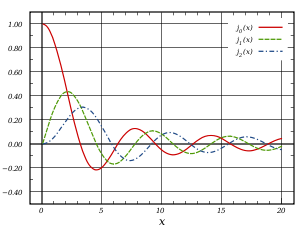
\includegraphics[height=0.3\textheight]{fig/bessel_j.png}
	\mycaption[Bessel function of the first kind - $J$]{Bessel function of the first kind - $J$.}
	\label{fig31}
\end{figure}


\begin{figure}[t!]
	\centering
	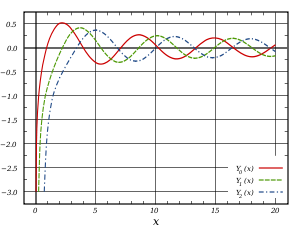
\includegraphics[height=0.3\textheight]{fig/bessel_y.png}
	\mycaption[Bessel function of the second kind - $Y$]{Bessel function of the second kind - $Y$.}
	\label{fig32}
\end{figure}

Consequently, the solution will be of the form $\rho(r) = AJ_0(\sqrt{\alpha}r) + CY_0(\sqrt{\alpha}r)$, $A$ and $C$ being constants.

We can now use boundary conditions. We know that the radial component of the flux has to be greater or equal to 0 $\forall r$. In our system, r = 0 at the center of the cylinder. However, $\lim_{r\to 0} Y_0(r) = -\infty$, implying that $C = 0$.

We also know that at a radius $R_e = R + \delta_e$, the flux is to be zero. Thus, $\phi(R_e) = 0$. So, we have to solve Equation~\ref{eq310}.

\begin{equation}\label{eq310}
AJ_0(\sqrt{\alpha}R_e) = 0
\end{equation}

This can be solved by A = 0, in which case we would obtain the trivial solution $\rho(r) = 0$, of no interest. $J_0(x) = 0$ can be verified for several $x$. However, since the flux has to be positive, the solution has to be the first zero of the function, happening for $x = 2.405$. Hence, Equation~\ref{eq310} is verified for $\sqrt{\alpha}R_e = 2.405$.

Thus, we have the solution of the radial component of the flux, presented in Equation~\ref{eq311}.

\begin{equation}\label{eq311}
\rho(r) = AJ_0(\frac{2.405}{R_e}r)
\end{equation}

Now, we can focus on the axial component of the flux, shown in Equation~\ref{eq38}. It is interesting to recognize in this equation the equation for an infinite slab geometry, for which the solution is known, explicited in Equation~\ref{eq312}.

\begin{equation}\label{eq312}
\zeta(z) = D\cos(\frac{\pi}{H_e}z)
\end{equation}

Finally, one can compute the flux $\phi(r, z)$, according to Equation~\ref{eq313}.

\begin{equation}\label{eq313}
\phi(r, z) = \phi_0 * J_0(\frac{2.405}{R_e}r)\cos(\frac{\pi}{H_e}z)
\end{equation}

Where $\phi_0 = A * D$.

We can also deduce the buckling $B^2 = \alpha + \beta = \left( \frac{2.405}{R_e} \right)^2 + \left( \frac{\pi}{H_e} \right)^2$.

\section{Radioactivity}
\label{prob32}

\subsection{Problem}
\textit{A radioactive sample is composed of two independently radioactive isotopes. A nuclear counter whose output is directly proportional to the total activity of the sample was used and gave the following count (Table 1-13,~\cite{book01}). Find the half-life and the decay constant of each of the two isotopes.}

\subsection{Solution}

The sample is composed of two independently radioactive isotopes. We assume that their respective hal-life is sufficiently different and low for one isotope contribution to be neglected after 26 hours. This means that after 26h, only one isotope, B, is contributing, as seen in Equation~\ref{eq314}.

\begin{equation}\label{eq314}
A(t) = A_{B, 0}e^{-\lambda_B t}
\end{equation}

Assuming that after 26 hours, the contribution comes only from isotope A implies that we can use the data points t=26h and t=28h to obtain a equations system. This system is needed to solve for $A_{B, 0}$ and for $\lambda_B$.

We can write Equations~\ref{eq315} and~\ref{eq316}.


\begin{equation}\label{eq315}
\lambda_B = \frac{\ln(1072/1010)}{3600 * (28-26)} = \text{\num{8.2744e-6}}
\end{equation}

\begin{equation}\label{eq316}
A_{B,0} = 1010 * e^{\lambda_B (28*3600)} = 842.4
\end{equation}

Consequently, the half-life of isotope B is $T_{1/2, B} = 23.27h$.

Subsituting the activity due to isotope B from the total measured, we can obtain the contribution of isotope C. Hence, $A(C, t=0) = 102000-842.4 = 101157.6$ and $A(C, t=4) = 26300 - A_{B, 0}e^{-\lambda_B 4*3600} = 25552$.

Hence, using Equation~\ref{eq317}, we can obtain.


\begin{equation}\label{eq317}
A(t) = A_{C, 0}e^{-\lambda_C t}
\end{equation}

And so,

\begin{equation}\label{eq318}
\lambda_C = \frac{\ln(101157.6/25552)}{3600 * 4} = \text{\num{9.555e-5}}
\end{equation}


Consequently, the half-life of isotope C is $T_{1/2, C} = 2.015h$. We can verify that after 10 periods of isotopes C half-life (21h), only the contribution of isotope B would remain. The calculation thus stands.

\section{Thermal fission factor}
\label{prob33}

\subsection{Problem}
\textit{Calculate the thermal-fission factor for 2200-m/sec neutrons for (a) natural uranium and for (b) 2 percent, (c) 20 percent, and (d) fully enriched uranium.}

\subsection{Solution}

The thermal fission factor, $\eta$, is described using Equation~\ref{eq319}.

\begin{equation}\label{eq319}
\eta = \frac{\nu\Sigma_f}{\Sigma_f + \Sigma_c} = \nu\frac{N_5\sigma_f^5}{N_5\sigma_f^5 + N_5\sigma_c^5 + N_8\sigma_c^8}
\end{equation}

Where:

\begin{conditions}
N_5 & Density of $U^{235}$ \\
N_8 & Density of $U^{238}$ \\
\sigma_f^5 & microscopic fission cross section of $U^{235}$ \\
\sigma_c^5 & microscopic capture cross section of $U^{235}$ \\
\sigma_c^8 & microscopic capture cross section of $U^{238}$
\end{conditions}

Knowing that the enrichment can be written $e = \frac{N_5}{N_5 + N_8}$, one can rewrite Equation~\ref{eq319} into Equation~\ref{eq320}.


\begin{equation}\label{eq319}
\eta = \nu\frac{e\sigma_f^5}{e\sigma_f^5 + e\sigma_c^5 + (1-e)\sigma_c^8}
\end{equation}


Considering $\nu = 2.43$, $\sigma_f^5 = 571.1\ b$, $\sigma_a^5 = \sigma_c^5 + \sigma_f^5 = 678.2\ b$ and $\sigma_c^8 = 2.73\ b$, the answers to \textit{(a), (b), (c)} and \textit{(d)} are respectively $1.30$, $1.71$,  $2.01$ and $2.05$.

\section{Cubical reactor core}
\label{prob34}

\subsection{Problem}
\textit{The extrapolation lengths in a cubical reactor core are negligibly small. Find the ratio of average to maximum flux if the flux distribution is:
(a) Sinusoidal in the x, y and z directions
(b) Sinusoidal in the x and y directions but uniform in the z direction
(c) Sinusoidal in the x direction only and uniform in the y and z directions.}

\subsection{Solution}

No fucking clue.


\section{Nuclear temperature coefficient}
\label{prob35}

\subsection{Problem}
\textit{Assuming constant $k_{\infty}$ and $B^2$, and a $1/V$ dependence of the thermal neutron absorption, show that the nuclear temperature coefficient in a thermal reactor is given by $\frac{\delta\rho_n}{\delta T} = - \frac{B^2 L^2}{2k_{\infty}T}$.}

\subsection{Solution}

We know that $L=\sqrt{\frac{d}{\Sigma_a}}$ and that $D = \frac{\lambda_{tr}}{3}$.

Consequently,

\begin{equation}\label{eq320}
L^2 = \frac{\lambda_a\lambda_{tr}}{3} = \frac{1}{3\Sigma_a\Sigma_s}
\end{equation}

In the $1/v$ region, v is proportional to $\sqrt{T}$. Consequently, $\sigma_a = \sigma_{a,0}\sqrt{\frac{T_0}{T}}$.

So, we can write $L^2 = L_0^2\sqrt{\frac{T_0}{T}}$.

Now, we can start from Equation~\ref{eq321}.


\begin{equation}\label{eq321}
k_{eff} = \frac{k_{\infty} l_f}{1 + L^2B^2}
\end{equation}

Knowing that $\rho = \frac{k_{eff} - 1}{k_{eff}}$, one can write:


\begin{equation}\label{eq322}
\rho = \frac{k_{\infty} - 1 - L^2B^2}{k_{\infty}}
\end{equation}

And so, plugging in $L^2$:


\begin{equation}\label{eq323}
\rho = \frac{k_{\infty} - 1}{k_{\infty}} - \frac{B^2L_0^2\sqrt{\frac{T}{T_0}}}{k_{\infty}}
\end{equation}

Derivative of this equation with regards to $T$ gives us:


\begin{equation}\label{eq324}
\frac{\delta \rho}{\delta T} = - \frac{B^2L_0^2(T T_0)^{-1/2}}{2k_{\infty}}
\end{equation}

The temperature coefficient at T is given for $T=T_0$, in which case:


\begin{equation}\label{eq325}
\frac{\delta \rho}{\delta T} = - \frac{B^2L^2}{2k_{\infty}T}
\end{equation}
